In this last chapter, we wrap up this work sharing conclusions. We also suggest new research lines inspired by the results of this work.

\section{Conclusions}

The main goal of this work was to evaluate the ability of classification models built from the topic modeling data, obtained by Latent Dirichlet Allocation. With a subset of documents, initial on time, called by \textit{Past}, we obtained their natural topics, then we do the same for intermediate data, called by \textit{Present}. After discovering the best correspondences for these topics, we built classification models for each one of them and evaluate the predictions over the years.

In chapter \ref{chap:intro}, we show a brief introduction, presenting the motivation and objective of this work. In chapter \ref{chap:literature} we described some important concepts of Natural Processing Language and classification techniques. In chapter \ref{chap:related} we presented related works that implement steps used in this work. 

Chapter \ref{chap:materials} described the whole methodology used to conduct the experimentation in this work, describing carefully each individual step. Finally, \ref{chap:results} presented and discussed the results obtained in each step of the experiment.

In synthesis, we saw from the results that are really possible to classify documents in short term, from a little subset of data. However, the topics evolve as time goes forward, evidenced by the discrepancy between the main closest correspondences and those that follow right away.

We identified two aspects of these classification models. Firstly, we have a tendency of constancy in the efficiency of the model, because of the slow evolution of a given subject, mostly when dealing with scientific publications, as in our case. The second aspect shows a decreasing trend over time, as the model tends to unlearn about themes as new terms are used, such as neural networks, for example, recently the use of deep learning for these kinds of applications has become very popular.

Given this decreasing aspect, our models gradually lose their ability to predict. Therefore, a re-train routine could be fundamental to always keep achieving good results.

\section{Future Work}

From now, we propose other research lines some improvements directly by the results previously obtained:

\begin{itemize}
	\item \textit{Forecast Step:}
	
	The immediate continuation given the chronological order is to develop the forecast step. Following the flowchart shown in Figure \ref{fig:forecast}, first, using the classifier we can build the incidence topic incidence matrix over time, with \textit{Past} and \textit{Present} sets. Then, apply a forecaster process for those time series with a regreesion technique, ideally using neural networks a Long Short-Term Memory neural network, \cite{hochreiter1997long}. Finally, with the \textit{Future} set, perform an evaluation for the built forecaster.
	
	\begin{figure}[h!]
		\centering
		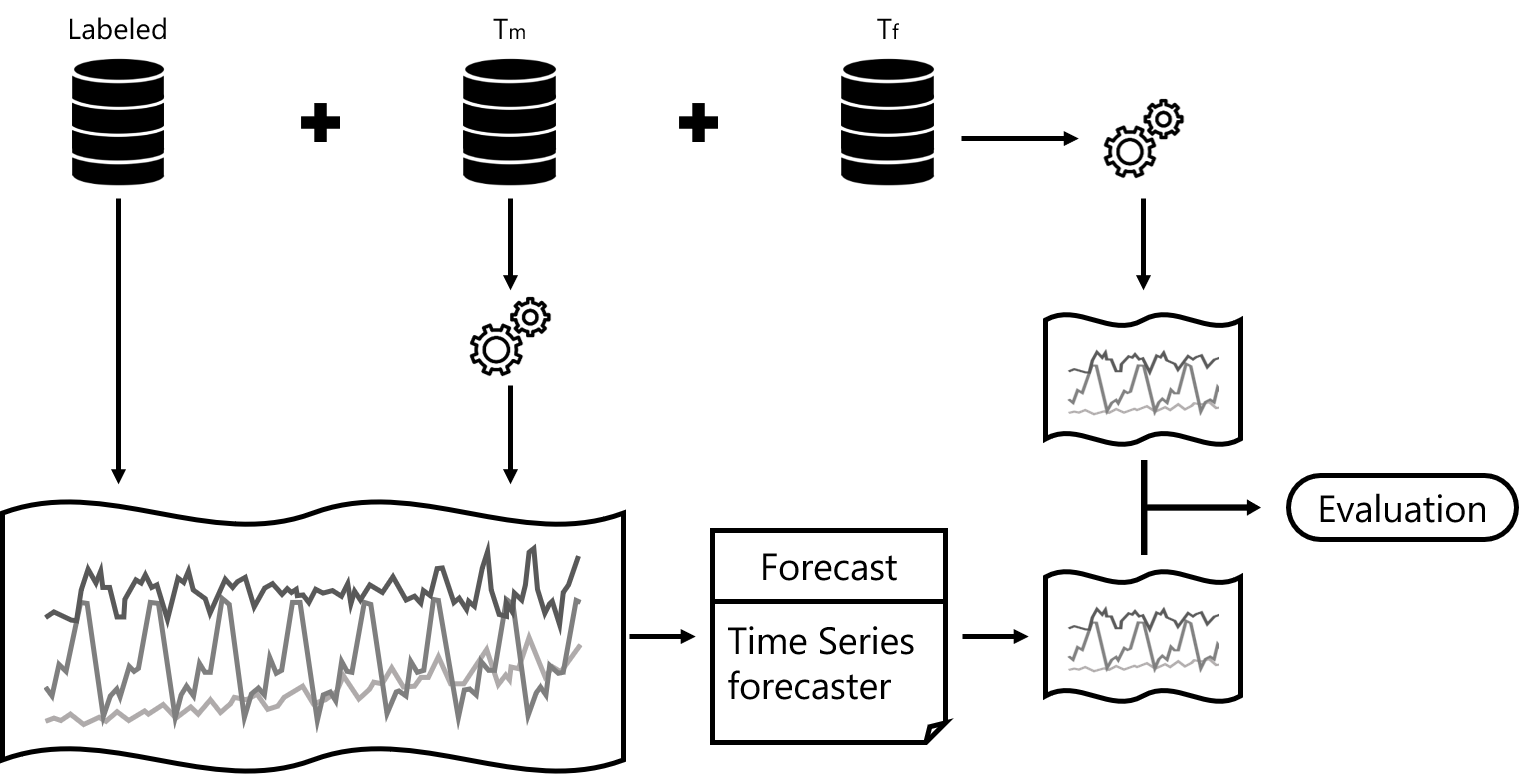
\includegraphics[width=0.8\linewidth]{01.Chapters/04.Materials/forecast}
		\caption{Flowchart to evaluate the time series model.}
		\label{fig:forecast}
	\end{figure}
	
	\item \textit{Retraining point:}
	
	Seeking to use this forecasting framework in a production environment, we will need to reduce the time granularity to month or even days. But, as we saw in Figure \ref{fig:isolated-topics} the classification models are losing efficiency over time. This research line aims to propose and evaluate metrics to identify an optimal threshold for retraining the topic model in order to update them with the new terms.
	
%	\item \textit{Topic modeling based on context:}
	
%	Text clusteing

	\newpage
	\item \textit{Feature extraction improvement:}
	
	In section \ref{sec:text-processing} we saw many techniques for normalization and vectorizing, but it does not stop there. Several unexplored techniques can improve our topic models and classification like n-grams.
	It is even possible to explore other metrics to better combine the past and present with topics such as cosine similarity.

	The word embedding itself presented a bad result, there are two possibilities to explain this. The first one consists of the algorithm used to train the classification Naive Bayes and SVM do not perform as well with embeddings so, a deep learning technique could be more appropriate to deal with embedding models. The second explanation could be due to the lack of a pre-trained model based on scientific publication context so, using a more appropriate embedding model could present a better result.
	
	It is even possible to improve the choice of threshold for the document to contain a class. For example, the majority class could be considered positive and use a higher threshold for the next ones.
	
	This research line aims to use more sophisticated techniques for improving the topic and classification models.
	
	
\end{itemize}
